
\documentclass[12pt]{article}
\usepackage{amsmath}
\DeclareMathOperator*{\argmin}{arg\,min} % thin space, limits underneath in displays
\DeclareMathOperator*{\argmax}{arg\,max} % thin space, limits underneath in displays
\newtheorem{thm}{Theorem}
\usepackage{amssymb}
\usepackage{amsfonts}
\usepackage{mathrsfs}
\usepackage{bm}
\usepackage{indentfirst}
\setlength{\parindent}{0em}
\usepackage[margin=1in]{geometry}
\usepackage{graphicx}
\usepackage{setspace}
\doublespacing
\usepackage[flushleft]{threeparttable}
\usepackage{booktabs,caption}
\usepackage{float}
\usepackage{graphicx}

\usepackage{import}
\usepackage{xifthen}
\usepackage{pdfpages}
\usepackage{transparent}

\newcommand{\incfig}[1]{%
\def\svgwidth{\columnwidth}
\import{./figures/}{#1.pdf_tex}
}


\usepackage{graphicx}
\usepackage{xspace,color}
\usepackage{url}
\usepackage{listings}


\lstset{commentstyle=\color{gray},keywordstyle=\color{black},
showstringspaces=false, basicstyle = \small
} %% basicstyle set fontsize
\lstnewenvironment{rc}[1][]{\lstset{language=R}}{}
\newcommand{\ri}[1]{\lstinline{#1}}  %% Short for 'R inline'



\lstdefinelanguage{language=R}{
numbers=left,
numberstyle=\footnotesize,
numbersep=1em,
xleftmargin=1em,
framextopmargin=2em,
framexbottommargin=2em,
showspaces=false,
showtabs=false,
showstringspaces=false,
frame=l,
tabsize=4,
}



\title{Linear Regression}
\author{Synferlo}
\date{May, 10}


\begin{document}
\maketitle
\newpage



\section{Simple Linear Regression}

\subsection{Estimation}

\begin{equation*}
 \widehat{y} =  \widehat{\beta_0} +  \widehat{\beta_1} x
\end{equation*}

\begin{equation*}
 \widehat{\beta_1} = \rho_{xy} \frac{s_{y}}{s_{x}},
 \text{ and }  \widehat{\beta_0} =  \overline{y} -  \widehat{\beta_1}
   \overline{x}
\end{equation*}

$  \overline{x},  \overline{y} $: sample means\\
$ s_{x}, s_{y} $: sample standard deviation\\
$ \rho_{xy} $: the estimate of correlation between $ X $ and $ Y $
based on the data.\\



\subsection{Statistical Inference}

\begin{table}[h!]
\begin{center}
	
\begin{threeparttable}
		\caption{Price and Volume (unnormalized result)}			

\begin{tabular}{lllll}
\\ [-1.8ex]
\hline
\hline \\[-1.8ex]
 & {\textbf {Coefs}} & {\textbf {SE}} & {\textbf {t-value}} & 
 {\textbf {p-value}}\\
\\ [-1.8ex]
\hline \\[-1.8ex]

 (Intercept) &2.342e+03  &8.799e+01   &26.62   &$<2e-16$ ***\\
 Volume      &2.696e-07  &5.252e-09   &51.33   &$<2e-16$ ***\\
\hline \\[-1.8ex]
Multiple R-squared:  &0.5061 &Adjusted R-squared:  &0.506\\
\\ [-1.8ex]
\hline \\[-1.8ex]

\end{tabular}
\begin{tablenotes}
\small
\item Signif. codes:  0 ‘***’ 0.001 ‘**’ 0.01 ‘*’ 0.05 ‘.’ 0.1 ‘ ’ 1\\
\item Residual standard error: 3803 on 2571 degrees of freedom\\
\item F-statistic:  2635 on 1 and 2571 DF,  p-value: $< 2.2e-16$\\
\end{tablenotes}


\end{threeparttable}
\end{center}
\end{table}



$ p $-value and $ t $-value for the coefs are the results of a two-
tailed test based on $ t $-distribution with DOF = 2.
\begin{align*}
H_0:& \beta_{j} = 0\\
H_1:& \beta_{j} \ne 0
\end{align*}

where $ j = 0 $ for the intercept $ \beta_0 $, and $ j = 1 $ for the
coef. of the volume.




\subsubsection{$ R^{2} $ and adjusted $ R^{2} $}

\begin{equation*}
R^{2} = \rho_{xy}^{2}
\end{equation*}

In R, 
\begin{rc}
# compute correlation then square it.
cor(df$Open_price, df$Volume, use = 'complete.obs')**2
# [1] 0.5061467
\end{rc}


You can check this 0.506 with the R-squared we've got from 
$ summary(result) $. They are exactly the same.



R-squared tells us 50 percent of the variation in the price can be 
attributed to volume.\\

The adjusted R-squared is important {\underline {ONLY IF}} you are
using the coef of determination to assess the overall quality of the
fitted model in terms of a balance between goodness of fit(GOF) and
complexity.



\subsubsection{Other summary output}
Residual standard error is the estimated SE of the $ \varepsilon $,
i.e., $  \widehat{\sigma} $.





\subsection{Categorical Predictor}

Explanatory variables can be categorical.

\subsubsection{Binary Variables}

\begin{equation*}
Y = \beta_0 + \beta_1 X + \varepsilon
\end{equation*}
X can be either 0 or 1.

If so, the interpretation of $ \beta $ would be different.
It's better to think of them like two {\underline {intercepts}},
where $ \beta_0 $ provides the {\underline {baseline}} of the response
when $ X = 0 $, and $ \beta_1 $ represents the {\underline {additive
effect}} on the mean response if $ X = 1 $.




\subsubsection{Multilevel variables}
The categorical variables have more than two levels.
For example, there can be many levels under education, e.g., 
high school, college, master, phd, etc.

Suppose there are $ k $ levels, then variable X can be written as
\begin{align*}
X &= 1,2,3,...,k\\
X_{(1)} = 0,1 \quad X_{(2)} &= 0,1 \quad ... X_{(k)} = 0,1
\end{align*}

And we can write the model,
\begin{equation*}
 \widehat{y} =  \widehat{\beta}_{0} +  \widehat{\beta}_{1}X_{(2)}
  +  \widehat{\beta}_{(2)}X_{(3)} + ... +  \widehat{\beta}_{k - 1}X_{(k)}
\end{equation*}

We normally use $ k - 1 $ of the dummy variables. Also,
each observation only satisfy one of the levels, i.e., if you are a
Ph.D. student, then you cannot be a high school student.
Hence, when $ X_{(i)} = 1 $, all others equals to zero.

So, if one observation belongs to level 3, then the model (
the predicted mean) would be
\begin{equation*}
 \widehat{y} =  \widehat{\beta}_{0} +  \widehat{\beta}2
\end{equation*}

Since the reference level(that omitted dummy) is defined as 1, 
if an observation has values of zero for all other dummies, it
implies the obs originally had X = 1.
\begin{equation*}
 \widehat{y} =   \widehat{\beta}_{0}
\end{equation*}
Here we have the result of a model with a dummy has four levels (
Heavy, Never, Occas, Regular), where Heavy is the reference.

\begin{figure}[H]
		\center{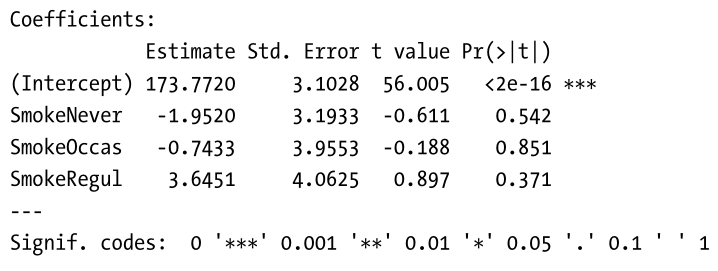
\includegraphics[scale =.7 ]  {figures/dummies_in_linear_model.png}}
\end{figure}



The observation in the reference category Heavy is represented solely
by $  \widehat{\beta}_{0} = 173.7720 $.




\section{Multiple Linear Regression}


\subsection{Terminology}

A {\underline {lurking variable}}, is what we've learned of the
{\underline {omitted variable}}. It can lead to a omitted variable bias.

A {\underline {nuisance or extraneous variable}} is a predictor of
no interest, but has the potential to confound (mess up) relationships
between other variables, and so affect your estimation. We are not
interested in it, but we {\underline {must}} add it to the model.


\subsection{The model}

\begin{equation*}
Y = \beta_0 + \beta_1 X_1 + \beta_2X_2 + ... + \beta_{p}X_{p} +
\varepsilon
\end{equation*}

You have $ n $ obs and $ p $ explanatory variables. For each obs, the
regression equation would be
\begin{equation*}
		y_{i} = \beta_0 + \beta_1x_{1,i} + \beta_2x_{2,i} + ... + 
		\beta_{p}x_{p,i} + \varepsilon_{i}
\end{equation*}
where $ i = 1,2,...,n $ stand for the $ i^{\text{ th }} $ obs.


{\textbf {Least-squared:}}
\begin{equation*}
\min_{\substack{\\}} \left( 
		\sum\limits_{i = 1} ^n(
		y_{i} - (\beta_0 + \beta_1x_{1,i} + \beta_2x_{2,i} + ... + 
		\beta_{p}x_{p,i})
		)	^{2}
\right)  
\end{equation*}


{\textbf {Matrix Form:}}
\begin{equation*}
\bm{Y} = \bm{X}\cdot \bm{\beta} + \bm{\varepsilon}
\end{equation*}
where $ \bm{Y} $ and $ \bm{\varepsilon} $ are $ n  \times 1 $ matrices
\begin{equation*}
\bm{Y} = 
\begin{bmatrix}
y_1\\y_2\\ \vdots  \\y_{n}
\end{bmatrix}
\quad
\text{ and }
\quad
\bm{\varepsilon} = 
\begin{bmatrix}
\varepsilon_1\\\varepsilon_2\\ \vdots  \\\varepsilon_{n}
\end{bmatrix}
\end{equation*}


\begin{equation*}
\bm{\beta} = 
\begin{bmatrix}
\beta_0\\\beta_1\\ \vdots \\\beta_{p}
\end{bmatrix}
\quad
\text{ and }
\quad
\bm{X} = 
\begin{bmatrix}
1 & x_{1,1} &\cdots&x_{p,1}\\
1 & x_{1,2} &\cdots&x_{p,2}\\
\vdots & \vdots &\ddots &\vdots \\
1 & x_{1,3} &\cdots&x_{p,3}\\
\end{bmatrix}
\end{equation*}


Matrix $ \bm{X} $ is $ n  \times (p + 1) $ dimension.


The OLS estimator $  \widehat{\bm{\beta}} $ :
\begin{equation*}
 \widehat{\bm{\beta}} = 
 \begin{bmatrix}
  \widehat{\beta}_{0}\\  \widehat{\beta}_{1}\\ \vdots \\  
	\widehat{\beta}_{p}
 \end{bmatrix}
 = (\bm{X}^{T}\cdot \bm{X})^{ - 1}\cdot \bm{X}^{T}\cdot \bm{Y}
\end{equation*}



\subsection{Interpretation of the coef}

A coefficient for a specific variable should be interpreted as the
change in the mean response for a one-unit increase in the variable,
while {\underline {holding all other variables constant}}.




\subsection{Transformation}

Two ways to approach the transformation: 
{\underline {polynomial}} and {\underline {logarithmic}}.

The transformation in general does not represent a universal solution
to solving problems of {\underline {nonlinearity}} in the trend,
but it can at least {\underline {improve}} how faithfully a linear
model is able to represent those trends.



\subsubsection{Polynomial}
Add squared, cubic, and other polynomial terms to fit curved trend.
For example, 
\begin{equation*}
\text{ Income } = \beta_0 + \beta_1edu + \beta_2edu^{2} + 
\beta_3 exp + \beta_4exp^{2} + \varepsilon
\end{equation*}

Use $ I() $ function in R to add a polynomial term in $ lm() $ function.

{\textbf {Code:}}
\begin{rc}
lm_poly_result = lm(norm_price~norm_volume+norm_supply
+I(norm_supply**2),data = df)
summary(lm_poly_result)
\end{rc}


If the effect of adding one term is not good, we can try to add another 
cubic term and compare these two models.






\begin{table}[h!]
\begin{center}
	
\begin{threeparttable}
		\caption{Quadratic vs. Cubic term model}			

\begin{tabular}{lllll}
\\ [-1.8ex]
\hline
\hline \\[-1.8ex]
 & {\textbf {Model 1}} & {\textbf {Model 2}}  \\
\\ [-1.8ex]
\hline \\[-1.8ex]


(Intercept)      	&-0.024260   			&-0.095378 ***	 \\
									&(-1.523)    			&( -5.557)    	\\
norm\_volume      & 0.465420***			& 0.418280 ***	 \\ 
									&(28.338)    			&( 24.920)    	\\
norm\_supply      & 0.397987***			& 0.525587 ***	 \\ 
									&(24.030)    			&( 25.473)    	\\
I($norm\_supply^2$) & 0.024269*  			& 0.088337 ***	 \\ 
									&( 2.446)    			&(  7.588)    	\\
I($norm\_supply^3$) &                 &-0.030171 ***	\\
				          &                 &(-10.035)    	\\


\\ [-1.8ex]
\hline \\[-1.8ex]

\end{tabular}
\begin{tablenotes}
\small
\item Signif. codes:  0 ‘***’ 0.001 ‘**’ 0.01 ‘*’ 0.05 ‘.’ 0.1 ‘ ’ 1\\
\end{tablenotes}

\end{threeparttable}
\end{center}
\end{table}



Now we can see, by adding cubic term, the model performs better.


\subsubsection{Logarithmic}
Transforming to a logarithmic scale can help reduce the severity of
heavily {\underline {skewed}} data.




\subsection{Interaction Terms}

When estimating regression models, you always have to accompany 
interactions with the {\underline {main effect}} of the relevant
predictors.

In R, use a ``:"  specify an interaction term.

{\textbf {Code:}}

\begin{rc}
inter_lm_result = lm(
		norm_price~norm_volume+norm_supply+norm_volume:norm_supply,
		data = df
)
summary(inter_lm_result)
\end{rc}





\section{Linear Model Selection}

\subsection{Goodness of fit vs. Complexity}
{\textbf {GOF:}} refers to the goal of obtaining a model that best 
represents the relationships between the dependent and explanatory 
variables.\\

{\textbf {Complexity: }} how many terms (e.g., polynomial, etc) and
additional functions in your model. The more you have, the more 
complex the model would be.\\


{\textbf {The principle of parsimony:}} 
The balancing act between GOF and complexity.\\
Our goal is to find a model that is as simple as possible without
sacrificing too much GOF.\\
The model satisfies this notion is a {\underline {parsimonious fit}}.





\subsubsection{General Guideline}

1. You CANNOT remove individual levels of a categorical variable in 
a given model. Suppose college, master, phd are under edu, but only
phd are significant. You cannot remove the college and master. 
You can ONLY remove the entire categorical variable, i.e., edu.\\

2. If an interaction term is present in the fitted model, ALL lower-
order interactions and main effects of the relevant variables MUST
remain in the model. Suppose you add an interaction term,
$ edu  \times exp  \times age $, then the main effect ($ edu, exp,
age$) and all lower-order interaction terms ($ edu  \times exp,
edu  \times age, exp  \times age$) should be shown in the model.
Hence, in R, you'd better use $ VR_1*VR_2 $ for interaction term, so
that R will add all these terms for you. You will not miss any one of
them.\\

3. Keep ALL lower-order polynomial terms in the model if the highest
is deemed significant.



\subsection{Model Selection Algorithms}

\subsubsection{Nested Comparisons: The Partial F-Test}

It is the most direct way to compare several different models.
It looks at two or more {\underline {nested}} models.
The less complex model is a reduced version of the more complex model.
\begin{align*}
 \widehat{y}_{\text{ redu }} =  \widehat{\beta}_{0} +  
 \widehat{\beta}_{1}x_1  +  \widehat{\beta}_{2}x_2 + ... +
 \widehat{\beta}_{p}x_{p}\\
 \widehat{y}_{\text{ full }} =  \widehat{\beta}_{0} +  
 \widehat{\beta}_{1}x_1  + ... + ... \widehat{\beta}_{p}x_{p} + 
 ... +  \widehat{\beta}_{q}	x_{q}
\end{align*}

Clearly, $  \widehat{y}_{\text{ full }} $ is more complex than
$  \widehat{y}_{\text{ redu }} $, so we say that 
$  \widehat{y}_{\text{ redu }} $ is {\underline {nested}} within
$  \widehat{y}_{\text{ full }} $.

The {\textbf {partial F-Test}} tries to answer if it is worth it
to include any additional variables. Its goal is to test whether
include those extra $ q - p $ terms in $  \widehat{y}_{\text{ full }} $
provide a statistically significant improvement GOF.

\begin{align*}
H_0:& \beta_{p + 1} = \beta_{p + 2} = ... = \beta_{q} = 0\\
H_1:& \text{ At least one of the } \beta_{j} \ne 0 (\text{ for }
j = p,...,q)
\end{align*}


If the $ p $-value is less than the significant level, then we say
it is worth it because at least one of those extra $ q - p $ terms
is non-zero.


$ F $ statistics:
\begin{equation*}
F = \frac{
		(R_{\text{ full }}^{2} - R^{2}_{\text{ redu }}(n - q - 1))
}
{(1 - R^{2}_{\text{ full }})(q - p)}
\end{equation*}

It follows an $ F $ distribution with $ df_1 = q - p $, 
$ df_2 = n - q $ degree of freedom. The $ p $-value is found as the
{\underline {upper-tail}} area from $ F $ as usual.

















\end{document}

